\subsection{Datenvorverarbeitung}
\glqq Da die Zieldaten aus den Datenquellen lediglich extrahiert werden, ist im Rahmen der Datenvorverarbeitung die Qualität des Zieldatenbestandes zu untersuchen und – sofern nötig – dieser durch den Einsatz geeigneter Verfahren zu verbessern.\grqq\seFootcite{}{S. 9}{Cleve.2014}

Diese essentielle Phase verfolgt das Ziel, die unstrukturierten und zunächst nutzlos scheinenden selektierten Rohdaten, in Daten höherer Qualität umzuwandeln, um diese der passenden \gls{dm}-Methode im geeigneten Format bereitstellen zu können. Die Struktur und das Format müssen perfekt auf die vorliegende Aufgabe passen, ansonsten führt die geringe Qualität der Daten zu schlechten bzw. falschen Resultaten, bis hin zu Laufzeitfehlern.\seFootcite{Vgl.}{S. 10-11}{Garcia.2015} Es gilt auch hier das alte Prinzip: GIGO – garbage in, garbage out.\seFootcite{Vgl.}{S. 197}{Cleve.2014} Die oftmals schlechte Qualität der (Roh-)Daten ist durch \textit{fehlende, ungenaue, inkonsistente bzw. widersprüchliche} Daten zu begründen.\seFootcite{Vgl.}{S. 84}{Han.2012}\seFootcite{Vgl.}{S. 196}{Cleve.2014} Im Folgenden werden dazu einige Ursachen beispielhaft aufgeführt.

Ungenaue bzw. falsche Daten können schon bei der Erhebung entstehen, wenn ein falsches Datenerhebungsinstrument ausgewählt wurde. Bei Stichproben sollte die Gesamtmenge so präzise wie möglich widergespiegelt werden, um die Datenakkuratesse nicht zu gefährden.\seFootcite{Vgl.}{S. 25}{Fahrmeir.2007} Weiterhin können technische und menschliche Fehler zu ungenauen Daten führen, indem Personen beispielsweise ihre persönlichen Informationen bei einer Befragung absichtlich verschleiern (z.B. Standardwert für Geburtsdatum 1. Januar), wobei man diese Problematik auch als \textit{\glqq disguised missing data\grqq}~bezeichnet.\seFootcite{Vgl.}{S. 84}{Han.2012}\seFootcite{Vgl.}{S. 24}{Fahrmeir.2007}\seFootcite{Vgl.}{S. 196}{Cleve.2014} Neben der falschen subjektiven Einschätzung des Menschen bei der Erhebung, können auch aus technischem Blickpunkt ungenaue Daten ermittelt werden, wie z.B. durch (teils-)defekte Sensoren. Nicht zuletzt können Daten bei einem Transfer verfälscht werden bzw. sogar teilweise verloren gehen.\seFootcite{Vgl.}{S. 84}{Han.2012}

Fehlende Daten lassen sich einerseits durch technische Mängel begründen, andererseits auch durch die Tatsache, dass bestimmte Attribute schlichtweg von Beginn aus bei der Erhebung nicht beachtet wurden oder durch bestimmte Restriktionen nicht verfügbar sind.\seFootcite{Vgl.}{S. 84-85}{Han.2012}

Die aufgezeigten Beispiele spiegeln nur einen kleinen Teil möglicher Ursachen wider und sollen die Bedeutsamkeit dieser Phase für den Data-Mining-Prozess aufzeigen. Die Datenvorbereitung stellt dabei einige mächtige Werkzeuge zur Verfügung, um die Datenqualität nachhaltig zu verbessern:\seFootcite{Vgl.}{S. 11 ff}{Garcia.2015}\seFootcite{Vgl.}{S. 196 ff}{Cleve.2014}\seFootcite{Vgl.}{S. 84 ff}{Han.2012}

\begin{itemize}
\item \textbf{Data Cleaning}: In diesem Schritt werden die Daten bereinigt, indem beispielsweise \textit{fehlerhafte} oder \textit{störende} Daten korrigiert werden (siehe \vref{dc}).

\item \textbf{Data Integration}: Diese Phase beschäftigt sich mit der fehlerfreien Zusammenführung von Daten, da diese oftmals aus mehreren unterschiedlichen Quellen stammen (siehe \vref{di}).

\item \textbf{Data Reduction}: Um die Algorithmen der Data Mining Methoden nutzen zu können, muss die immense Datenmenge reduziert bzw. komprimiert werden, um lange Laufzeiten zu verhindern (siehe \vref{dr}).
\end{itemize}

Auf die in \vref{werkzeuge} vereinfacht, dargestellten Werkzeuge und ihre Konzepte, wird in den folgenden Unterkapitel näher eingegangen.

\begin{figure}[H]
\centering
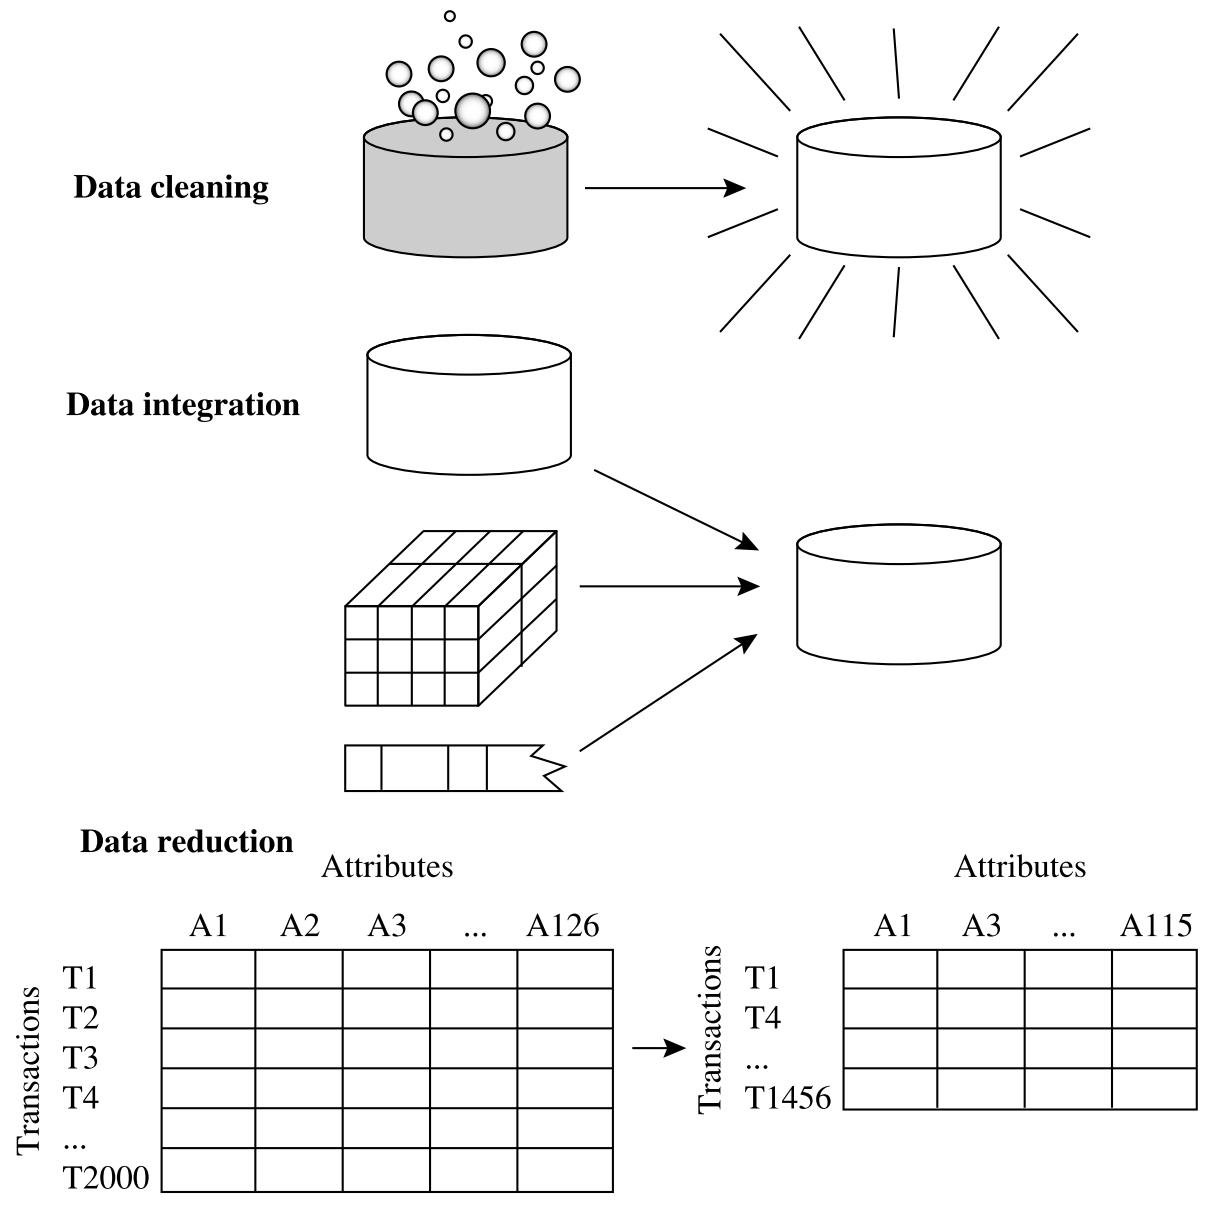
\includegraphics[scale=1.2]{se-wa-jpg/preprocessing}
\caption[Werkzeuge der Datenvorverarbeitung]{Werkzeuge der Datenvorverarbeitung\protect\footnotemark}
\label{werkzeuge}
\end{figure}
\footnotetext{Vgl. Abbildung \textit{Han}, Data Mining: Concepts and techniques, 2012, S. 87}


\subsubsection{Data Cleaning}
\label{dc}
In der realen Welt sind Daten häufig \glqq unvollständig, mit Fehlern oder Ausreißern behaftet oder sogar inkonsistent.\grqq\seFootcite{}{S. 199}{Cleve.2014} Um Fehler oder gar falsche Resultate im Data-Mining-Prozess frühzeitig zu vermeiden, ist es von großer Bedeutung, die Datenmengen zu bereinigen. Der Fokus sollte hierbei auf der Informationsneutralität liegen. Das heißt, es sollen möglichst keine neuen Informationen hinzugefügt werden, die das reale Abbild verzerren oder verfälschen könnten.\seFootcite{Vgl.}{S. 199-200}{Cleve.2014} Folgende Problemarten gilt es zu behandeln:

\paragraph{Fehlende Daten} 
Dem Datenanalyst stehen einige Möglichkeiten zur Verfügung, um auf fehlende Daten reagieren zu können:\seFootcite{Vgl.}{S. 88-90}{Han.2012}\seFootcite{Vgl.}{S. 200-201}{Cleve.2014}

\begin{itemize}
\item \textit{Attribut ignorieren}
\\ Der Datensatz mit dem fehlenden Attribut wird gänzlich ignoriert oder gelöscht. Jedoch können dadurch wichtige Informationen für die Datenanalyse verloren gehen, wodurch dieses Verfahren nur bei Datensätzen mit mehreren Lücken angewandt werden sollte.

\item \textit{Manuelles Einfügen}
\\ Besitzt der Datenanalyst das nötige Wissen, kann dieser einzelne Datensätze nachträglich manuell einfügen. Dieser Vorgang entwickelt sich schnell zu einem sehr zeitaufwändigen und unrealistischen Vorgang, der aufgrund des Mangels an Ressourcen (personeller wie auch zeitlicher) undurchführbar ist, sobald die Datenmenge wächst (z.B. 500 Kundendaten per Hand nachtragen).

\item \textit{Globale Konstante}
\\ Den fehlenden Wert durch eine globale Konstante zu ersetzen, ist sinnvoll, wenn auch ein leeres Feld als Information angesehen wird. Beispiele für Konstanten wären \textit{unbekannt} oder \textit{minus unendlich}.

\item \textit{Durchschnittswert}
\\ Handelt es sich bei dem fehlenden Attribut um einen metrischen Wert, so kann der Durchschnittswert aller Einträge als Ersatz verwendet werden. Der Durchschnittswert zeigt sich als äußerst einfache Möglichkeit, wenn die Daten klassifiziert werden können und dadurch die Durchschnittswertberechnung nur auf Datensätzen der selben Klasse angewandt wird. Die Methode der \gls{knn}\seFootcite{Vgl.}{S. 76}{Garcia.2015} steht zur Verfügung, wenn keine Klassen vorhanden sind. Hierbei wird der Durchschnitt, der dem aktuellen Datensatz ähnlichsten Werte benutzt wird.

\item \textit{Wahrscheinlichster oder häufigster Wert}
\\ Durch statistische Methoden kann der wahrscheinlichste Wert für das fehlende Attribut ermittelt werden, jedoch sollte diese Angleichung begründet sein. Bei nicht numerischen Werten kann als weitere Möglichkeit auch der häufigste Wert, als Ersatz für das fehlende Attribut verwendet werden.
\end{itemize}

\paragraph{Verrauschte Daten und Ausreißer}
Durch ungenaue Messwerte oder falschen Schätzungen entstehen die sogenannten \textit{verrauschten Daten}.\footnote{Im englischen Sprachgebrauch als \textit{noisy data} bekannt.} Um diese bereinigen zu können, stehen dem Datenanalyst einige Verfahren zur Verfügung, wodurch diese fehlerbehafteten Daten angeglichen werden können.\footnote{Auch als \textit{smoothing} bekannt.} Als \textit{Ausreißer} bezeichnet man dabei Daten, die erheblich von den anderen Daten abweichen oder außerhalb eines Wertebereiches liegen.\seFootcite{Vgl.}{S. 89-90}{Han.2012} Beispielsweise liegen Daten von 30- bis 50- Jährigen vor, darunter auch einer von einem 90-Jährigen. Hierbei könnte es sich um einen Ausreißer handeln, aber auch um einen fehlerhaften Datensatz.\seFootcite{Vgl.}{S. 196}{Cleve.2014} \glqq Ob solche Ausreißer für das Data Mining ausgeblendet oder adaptiert werden sollten oder besser doch im Originalzustand zu verwenden sind, hängt vom konkreten Kontext ab.\grqq\seFootcite{}{S. 196}{Cleve.2014}


\begin{itemize}

\item \textit{Klasseneinteilung (bining)}
\\ Durch die Gruppierung verrauschter Daten in Klassen, können diese beispielsweise durch den Mittelwert oder die naheliegenden Grenzwerte ersetzt werden. 

\item \gls{regression}
\\ Die Darstellung der Daten in Form einer mathematischen Funktion, bietet die Möglichkeit, fehlerbehaftete Daten  durch die berechneten Funktionswerte zu ersetzen. Für zwei Abhängigkeiten zwischen zwei Attributen steht hierbei neben der \textit{linearen Regression}, auch die \textit{multiple lineare Regression} für mehrere Attribute als Werkzeuge zur Verfügung. (weiterführende Ausarbeitung zur Regressionsanalyse siehe \vref{ra})

\item \textit{Verbundbildung (clustering)}
\\ Eine der einfachsten Möglichkeiten um Ausreißer zu erkennen, bietet die Verbundbildung, auch \gls{clustering} genannt. Hierbei werden ähnliche Daten, wie in \vref{outlier} dargestellt, zu \textit{Clustern} zusammengeführt, wodurch sich die Ausreißer direkt identifizieren lassen.

\begin{figure}[H]
\centering
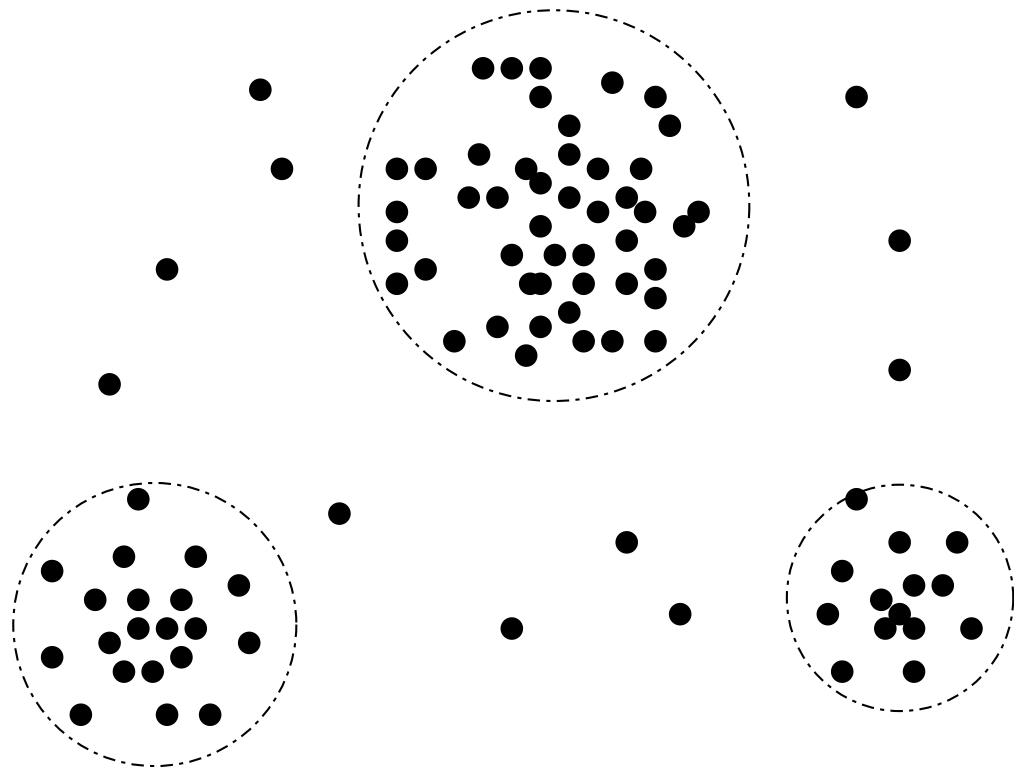
\includegraphics[scale=1.2]{se-wa-jpg/outlier}
\caption[Outlierdetection mittels Clustering]{Outlierdetection mittels Clustering\protect\footnotemark}
\label{outlier}
\end{figure}
\footnotetext{Vgl. Abbildung \textit{Han}, Data Mining: Concepts and techniques, 2012, S. 91}
\end{itemize}

\paragraph{Falsche und inkonsistente Daten}
Bei falschen bzw. inkonsistenten Daten ergeben sich prinzipiell zwei Möglichkeiten zur Korrekturbehandlung. Einerseits können der Datensatz oder bestimmte Attribute durch \textit{Löschen} entfernt werden, wobei jedoch die Gefahr einer zu großen Reduktion des Datenbestandes entsteht und relevante Informationen für das Data Mining verloren gehen könnten. Die zweite Korrekturvariante versucht den inkonsistenten Datensatz, durch die \textit{Zuhilfenahme anderer Datensätze}, sinnvoll zu ersetzen. Sollte eine Unterscheidung zwischen \textit{falsch} und \textit{richtig} nicht möglich sein, wären beim Löschen immer mindestens zwei Datensätze betroffen.\seFootcite{Vgl.}{S. 203-204}{Cleve.2014}

\subsubsection{Data Integration}
\label{di}
Bei Data-Mining-Projekten ist die Integration mehrerer Datenbestände aus unterschiedlichen Quellen oftmals erforderlich. Diese Phase sollte mit äußerster Sorgfalt durchgeführt werden, um frühzeitig redundante und inkonsistente Datensätze zu vermeiden, wodurch die Genauigkeit und Geschwindigkeit der nachfolgenden Data Mining Algorithmen nicht gefährdet wird.\seFootcite{Vgl.}{S. 93-94}{Han.2012} Folgende Punkte gilt es bei der Datenintegration zu beachten:

\begin{itemize}
\item \textbf{Identifikationsproblem von Entitäten}:
\\ Bei der Datenintegration aus multiplen Datenquellen, wie beispielsweise Datenbanken oder Dokumenten, stellt die Schema-Integration als auch die Objektanpassungen eine schwierige Herausforderung dar. Der Datenanalyst muss sicherstellen, dass zum Beispiel das Attribut \textit{kunden\_nummer} aus der einen Datenquelle, die selbe Referenz besitzt, wie das Attribut \textit{kunden\_id} aus einer Anderen und es sich folglich um das selbe Attribut handelt. Dies wird allgemein als \textit{Problem Identification Problem} bezeichnet.\seFootcite{Vgl.}{S. 199}{Cleve.2014}\seFootcite{Vgl.}{S. 94}{Han.2012}  Die Metadaten der Attribute beinhalten Informationen, wie \textit{Name, Bedeutung, Datentyp, Wertebereich, uvm.} und können durch einen Abgleich zu einer hilfreichen Vermeidung von Fehlern bei der Integration beitragen. Weiterhin muss gesondert auf die \textit{Datenstruktur} geachtet werden, um keine referentiellen Abhängigkeiten bzw. Beziehungen zwischen den Daten zu zerstören.\seFootcite{Vgl.}{S. 94}{Han.2012} 

\item \textbf{Redundanzen bei Attributen}:
\\ Ein Attribut, welches durch ein anderes Attribut ableitbar ist -- wie zum Beispiel das Alter vom Geburtsjahr berechnet werden kann -- wird als redundant bezeichnet. Die Vielzahl von Redundanzen führt zu unnötig aufgeblähten Datenmengen, die wiederum die Performanz sowie die Resultate eines Data Mining Algorithmus negativ beeinträchtigen können.\seFootcite{Vgl.}{S.41}{Garcia.2015} Folglich sollte diese Problematik mit zur Hilfenahme von statistischen Verfahren, in Form der Korrelationsanalyse, dezidiert behandelt werden. Für numerische Wert ist dabei der Einsatz von Korrelationskoeffizienten und Kovarianzen typisch. Um die Implikation zweier Attribute einer nominalen Datenmenge\footnote{Rein qualitative Merkmalsausprägungen ohne natürliche Rangordnung (wie z.B. das Geschlecht).} bestimmen zu können, verwendet man in der Regel den $\chi^2$(\textit{Chi})-Test.\seFootcite{Vgl.}{S. .}{Han.2012}\seFootcite{Vgl.}{S. 41}{Garcia.2015}\seFootcite{Vgl.}{S. 64}{Cleve.2014} 

\item \textbf{Duplikatserkennung}:
\\ Duplikate verkörpern Redundanzen auf Datensatzebene und führen einerseits zu unnötig großen Datenmengen, die sich wiederum auf die Performanz der Algorithmen auswirken, andererseits jedoch auch, durch die verfälschte Gewichtung der mehrfach vorkommenden Datensätze, zu schlichtweg falschen Analyseergebnissen führen kann. Ein häufiger Grund stellt dabei die Verwendung von denormalisierten Datenbanktabellen dar.\seFootcite{Vgl.}{S. 98}{Han.2012}\seFootcite{Vgl.}{S. 43}{Garcia.2015}

\item \textbf{Konflikte bei Attributswerten}:
\\ Hierbei handelt es sich um die unterschiedliche Darstellung, Skalierung und Kodierung von Attributswerten. Beispielsweise kann das Attribut \textit{Gewicht} durch das metrische System oder das britische Maßsystem repräsentiert werden, wodurch bei der Integration von Daten zu einer einheitlichen Quelle immer wieder Konflikten resultieren.\seFootcite{Vgl.}{S. 99}{Han.2012}\seFootcite{Vgl.}{S. 199}{Cleve.2014} 
\end{itemize}

\subsubsection{Data Reduction}
\label{dr}
Wie schon einige Male zuvor erwähnt wurde, umfassen Data-Mining-Aufgaben in der Regel riesige Datenmengen mit Millionen von Datensätzen, die die Komplexität und Effizienz der Algorithmen stark negativ beeinflussen. Daher strebt die Datenreduktion -- wie in der Bezeichnung zu erkennen -- nach einer reduzierten repräsentativen Teilmenge, welche die Integrität des Original nicht verliert. Dazu können folgende drei Techniken angewandt werden, die anschließend näher beleuchtet werden:\seFootcite{Vgl.}{S. 147 ff}{Garcia.2015}\seFootcite{Vgl.}{S. 99-100}{Han.2012}\seFootcite{Vgl.}{S. 206-208}{Cleve.2014} 

\begin{enumerate}

\item Dimensionsreduktion 

\item Datenkompression

\item Numerische Datenreduktion

\end{enumerate}

\paragraph{Dimensionsreduktion}
Hierbei bleiben irrelevante Attribute des Datensatzes unberücksichtigt und nur für die Analyse relevante Daten mit einbezogen. Allgemein empfehlen sich dafür zwei Verfahren. Bei der schrittweisen \textit{Vorwärtsauswahl} werden wesentliche Attribute einer sukzessiv wachsenden Zielmenge zugeordnet. Im Gegensatz dazu werden bei der \textit{Rückwärtseliminierung} die unwichtigen Daten schrittweise aus der Zielmenge herausgelöscht.\seFootcite{Vgl.}{S. 206}{Cleve.2014} 

\paragraph{Datenkompression}
\label{datenkompression}
Bei dieser Technik wird durch Transformation oder Codierung versucht eine Reduktion der Datenmenge zu erreichen. Fasst man beispielsweise die einzelnen Attribute \textit{Tag, Monat und Jahr} zu einem neuen Attribut \textit{Datum} zusammen, können Datensätze komprimiert werden.\seFootcite{Vgl.}{S. 207}{Cleve.2014}
 
\paragraph{Numerische Datenreduktion}
Statt die gesamte Datenmenge für die Analyse heran zunehmen, wird innerhalb der numerischen Datenreduktion eine repräsentative Teilmenge -- in Form einer Stichprobe -- für das \gls{dm} genutzt. Im Vordergrund steht hierbei die passende Auswahl unterschiedlicher Stichprobenverfahren, wie der \textit{zufällige Stichprobe} oder der \textit{repräsentative Stichprobe}, wobei keine Verzerrung der Realität resultieren darf.\seFootcite{Vgl.}{S. 25-27}{Fahrmeir.2007}\seFootcite{Vgl.}{S. 207}{Cleve.2014}